
\chapter{Implementation of a Poisson solver}
\label{chapter:poisson}

The aim of this chapter is to introduce the classes that make up the
foundation of Jive. To this end, it walks you through an example
program that uses the finite element method to compute the solution of
a Poisson problem. The example program demonstrates how to build a
finite element mesh; how to convert the PDE describing the Poisson
problem into a linear system of equations; and how to solve that
system of equations.

\BlankLine
This chapter starts with a brief description of the Poisson problem
and its boundary conditions.
Section~\ref{section:poisson:solution-procedure} then describes
how the Poisson problem can be solved by means of the finite element
method. This section also introduces some of the terminology that is
used in the remaining sections.  After that,
Section~\ref{section:poisson:class-summary} provides a summary
of the classes from Jive and Jem that are used in the example program.
The aim of this section is to reduce the amount of new information
that is presented in the following sections.
Section~\ref{section:poisson:program-structure} then summarizes
the structure of the example program. Next,
Sections~\ref{section:poisson:mesh-construction}
to~\ref{section:poisson:solution} describe how the example
program builds a mesh, assembles the linear system of equations, and
solves that system of equations.
Section~\ref{section:poisson:complete-program} ends this
chapter by listing the main function of the example program.

\BlankLine
The Poisson problem is defined on a two-dimensional, rectangular
domain~$\Omega$ with boundary $\Gamma = \DirichletBoundary \cup
\NeumannBoundary$, as illustrated in Figure~\ref{fig:poisson-problem}.
Homogeneous Dirichlet boundary conditions are prescribed
on~\DirichletBoundary, while homogeneous Neumann boundary conditions
are prescribed on~\NeumannBoundary. The mathematical formulation of
the problem is given by the following three equations:
\begin{displaymath}
  \begin{alignedat}{2}
    - \nabla^{2} u(\bm{x}) & = f(\bm{x}) \, , \qquad
      & \bm{x} & \in \Omega. \\
    u(\bm{x}) & = 0 \, , \qquad
      & \bm{x} & \in \DirichletBoundary. \\
    \bm{n} \Inproduct \bm{\nabla} u(\bm{x}) & =  0 \, , \qquad
      & \bm{x} & \in \NeumannBoundary.
  \end{alignedat}
\end{displaymath}
where the scalar $u$ is the state variable, $\bm{x}$ is the spatial
coordinate, $\Nabla$ is the gradient operator, and $f$ is a given
function. The vector~$\bm{n}$ is the normal on the Neumann
boundary~\NeumannBoundary.
\begin{Figure}

  \begin{center}
    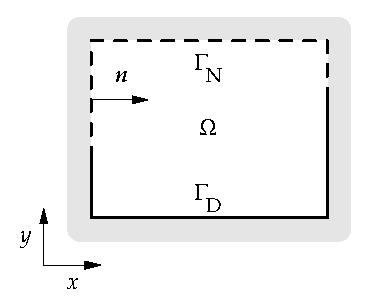
\epsfig{file=figures/poisson-problem.eps}
  \end{center}

  \caption{A schematic representation of the Poisson problem. The
    symbol~$\Omega$ denotes the spatial domain,
    \DirichletBoundary~denotes the Dirichlet boundary,
    \NeumannBoundary~denotes the Neumann boundary, and $\bm{n}$
    denotes the normal vector on~\NeumannBoundary.}

  \label{fig:poisson-problem}

\end{Figure}


%======================================================================

\section{The solution procedure}
\label{section:poisson:solution-procedure}

To solve the Poisson problem by means of the finite element method,
the PDE is first replaced by its equivalent weak formulation: find the
state $u$ such that
\begin{displaymath}
  \Int{\Omega} v \nabla^{2} u \, \Dee\Omega +
  \Int{\Omega} v f \, \Dee\Omega = 0
\end{displaymath}
for all continuous test functions $v$ which are zero
on~\DirichletBoundary. Using the divergence theorem, the weak
formulation can also be written as: find $u$ such that
\begin{displaymath}
  - \Int{\Omega} \Nabla v \Inproduct \Nabla u \, \Dee\Omega +
  \Int{\Omega} v f \, \Dee\Omega = 0
  \label{eq:poisson-weak}
\end{displaymath}
For all continuous test functions $v$.


%----------------------------------------------------------------------

\Signpost{Approximation by polynomial functions}

The next step in the finite element method is to approximate the state
$u$ by a set of polynomial functions. This is done by creating a
\emph{mesh} comprising a set of \emph{elements} and \emph{nodes}. The
elements -- numbered from one to~$n_e$ -- are obtained by dividing the
spatial domain~$\Omega$ into sub-domains $\Omega_{e_i}, i \in \{1,
\ldots, n_e\}$, as is illustrated in Figure~\ref{fig:poisson-mesh}.
The nodes -- numbered from one to~$n_n$ -- are obtained by defining a
set of points on the edges of the elements. Or, stated differently,
each element is assigned a set of nodes which it shares with other
elements.
\begin{Figure}

  \begin{center}
    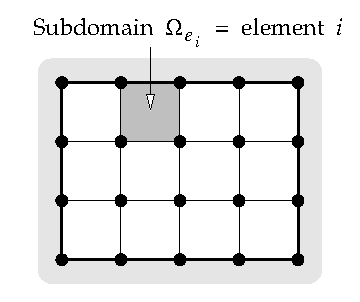
\epsfig{file=figures/poisson-mesh.eps}
  \end{center}

  \caption{A sample mesh for the Poisson problem.}

  \label{fig:poisson-mesh}

\end{Figure}

\BlankLine
In each element~$i$, the solution of the Poisson problem is
approximated by a polynomial function~$\hat{u}$ that is given by:
\begin{displaymath}
  \hat{u}(\bm{x}) = \bm{N}_{e_i}(\bm{x}) \, \bm{a}_{e_i} \, , \ \bm{x}
  \in \Omega_{e_i}.
\end{displaymath}
The matrix $\bm{N}_{e_i}$ contains the interpolation polynomials, or
\emph{shape functions}, of element~$i$.  Its dimensions are $1 \times
|e_i|$, where $|e_i|$ denotes the number of degrees of freedom
attached to element~$i$ (which, in this particular case, equals the
number of nodes attached to element~$i$).  The vector $\bm{a}_{e_i}$
contains the (unknown) values of the state in the nodes of the
element.

If the values of the state in all nodes of the mesh are collected in
one large vector~$\bm{a}$, then the above equation can also be written
as:
\begin{displaymath}
  \hat{u}(\bm{x}) = \bm{N}_{e_i}(\bm{x}) \, \bm{L}_{e_i} \bm{a}
  \, , \qquad \bm{x} \in \Omega_{e_i}.
\end{displaymath}
The matrix $\bm{L}_{e_i}$ is a sparse, boolean matrix with dimensions
are $|e_i| \times n_n$. It is called the \emph{location operator} of
element~$i$ because it extracts an element vector from a global
vector. That is, it extracts a vector defined on the nodes of an
element from a vector defined on all nodes of the mesh.

An approximation of $\Nabla u$ can be obtained by applying the
gradient operator to the previous equation. This yields:
\begin{equation}
  \Nabla \hat{u}(\bm{x}) = \bm{G}_{e_i}(\bm{x}) \, \bm{L}_{e_i} \bm{a}
  \, , \qquad \bm{x} \in \Omega_{e_i}
  \label{eq:poisson-gradient-approximation}
\end{equation}
where the matrix $\bm{G}_{e_i}$ contains the spatial derivatives of the
element shape functions. It has $|e_i|$ columns and as many rows as
the number of spatial dimensions (two in this case).

The test functions~$v$, which are used in the weak formulation, are
constructed in the same way as the approximate solution~$\hat{u}$.
This means that within each element~$i$
\begin{displaymath}
  v(\bm{x}) = \bm{N}_{e_i}(\bm{x}) \, \bm{L}_{e_i} \bm{w} \, ,
  \qquad \bm{x} \in \Omega_{e_i}
\end{displaymath}
where the global vector~$\bm{w}$ contains the values of the test
functions within the nodes of the mesh. The gradient of the test
functions are obtained simply by replacing the matrix $\bm{N}_{e_i}$
by the matrix $\bm{G}_{e_i}$.


%----------------------------------------------------------------------

\Signpost{Transformation into a system of equations}

The Poisson problem is now transformed into a linear system of
equations by substituting the polynomial approximations
into the weak formulation~(\ref{eq:poisson-weak}) of the Poisson
problem. This yields:
\begin{eqnarray*}
  - \Int{\Omega} \Nabla v \Inproduct \Nabla u \Dee\Omega +
  \Int{\Omega} v f \, \Dee\Omega
  & \approx & \\
  \sum_{i = 1}^{n_e} \left(
    - \Int{\Omega_{e_i}} \Nabla v \Inproduct \Nabla \hat{u} \,
    \Dee\Omega +
    \Int{\Omega_{e_i}} v f \, \Dee\Omega
  \right) & = & \\
  \sum_{i = 1}^{n_e} \left(
    - \Int{\Omega_{e_i}} (\bm{G}_{e_i} \bm{L}_{e_i} \bm{w})^{T}
    \bm{G}_{e_i} \bm{L}_{e_i} \bm{a} \, \Dee\Omega +
    \Int{\Omega_{e_i}} \bm{N}_{e_i} \bm{L}_{e_i} \bm{w} f \, \Dee\Omega
  \right) & = & \\
  \bm{w}^T \sum_{i = 1}^{n_e} \left(
    - \Int{\Omega_{e_i}} \bm{L}_{e_i}^{T} \bm{G}_{e_i}^{T}
    \bm{G}_{e_i} \bm{L}_{e_i} \, \Dee\Omega \, \bm{a} +
    \Int{\Omega_{e_i}} \bm{L}_{e_i}^{T} \bm{N}_{e_i}^{T} f \,
    \Dee\Omega
  \right) & = & 0
\end{eqnarray*}
Since the above equality must hold for all possible vectors~$\bm{w}$,
the final expression between the brackets must be equal to zero.
This means that the vector~$\bm{a}$ is the solution of
\begin{displaymath}
  \left(
    \sum_{i = 1}^{n_e} \Int{\Omega_{e_i}}
    \bm{L}_{e_i}^{T} \bm{G}_{e_i}^{T} \bm{G}_{e_i} \bm{L}_{e_i} \,
    \Dee\Omega
  \right) \bm{a} =
  \sum_{i = 1}^{n_e} \bm{L}_{e_i}^{T} \left(
    \Int{\Omega_{e_i}} \bm{N}_{e_i}^{T} \, f \, \Dee\Omega
  \right)
\end{displaymath}
which can be written as
\begin{equation}
  \bm{K} \bm{a} = \bm{f}.
  \label{eq:poisson-linear-system}
\end{equation}
The matrix $\bm{K}$ is a $(n_n \times n_n)$ sparse matrix that is
called the \emph{global matrix}. It is assembled element-wise as
follows:
\begin{displaymath}
  \bm{K} = \sum_{i = 1}^{n_e} \bm{L}_{e_i}^{T} \left(
    \Int{\Omega_{e_i}} \bm{G}_{e_i}^{T} \bm{G}_{e_i} \, \Dee\Omega
  \right) \bm{L}_{e_i} =
  \sum_{i = 1}^{n_e} \bm{L}_{e_i}^{T} \bm{K}_{e_i}
  \bm{L}_{e_i}.
\end{displaymath}
The matrix~$\bm{K}_{e_i}$ is a $(|e_i|\times |e_i|)$ dense matrix that
is called the \emph{element matrix} of the $i$-th element. The
vector~$\bm{f}$ has length $n_n$ and is called the \emph{global
  right-hand side} vector. Like the global matrix it is constructed
element-wise:
\begin{equation}
  \bm{f} = \sum_{i = 1}^{n_e} \bm{L}_{e_i}^{T} \left(
    \Int{\Omega_{e_i}} \bm{N}_{e_i}^{T} \, f \, \Dee\Omega
  \right)
  = \sum_{i = 1}^{n_e} \bm{L}_{e_i}^{T} \, \bm{f}_{e_i}.
  \label{eq:global-righ-hand-size}
\end{equation}
The vector $\bm{f}_{e_i}$ is called the \emph{element right-hand side}
vector of the $i$-th element. Its length is equal to $|e_i|$.

\BlankLine
Since the solution of the Poisson problem must satisfy the Dirichlet
boundary conditions, all components of $\bm{a}$ corresponding with the
nodes on the Dirichlet boundary must be equal to zero. If these
prescribed components are numbered last, then the system of
equations~(\ref{eq:poisson-linear-system}) can be written as:
\begin{displaymath}
  \left[
    \begin{array}{cc}
      \bm{K}_{11} & \bm{K}_{12} \\
      \bm{K}_{21} & \bm{K}_{22}
    \end{array}
  \right] \left[
    \begin{array}{c}
      \bm{a}_{1} \\
      \bm{0}
    \end{array}
  \right] = \left[
    \begin{array}{c}
      \bm{f}_{1} \\
      \bm{f}_{2}
    \end{array}
  \right]
\end{displaymath}
in which the vector $\bm{a}_{1}$ contains all unknown, non-prescribed
components of $\bm{a}$. The unknown components are therefore obtained
by calculating the solution of
\begin{displaymath}
  \bm{K}_{11} \, \bm{a}_{1} = \bm{f}_{1}.
\end{displaymath}


%======================================================================

\section{Outline of the program}
\label{section:poisson:program-outline}


%======================================================================

\section{Construction of the mesh}
\label{section:poisson:mesh-construction}


%======================================================================

\section{Assembly of the global system of equations}
\label{section:poisson:assembly}


%======================================================================

\section{Solution of the global system of equations}
\label{section:poisson:solution}


%======================================================================

\section{The complete program}
\label{section:poisson:complete-program}
